\documentclass[11pt]{article}
\usepackage{mathblatt}
\usepackage{adjustbox,varwidth}
% gesetzt von werkzeuge/setzer.py; Lösungen nach bau/bauregeln.md „Lösungen“.
\newcommand{\kennung}{XKT}
\begin{document}
\pfheftstil
\fancyfoot[C]{{\footnotesize\color{mbgrau}\kennung\hfill\thepage}}
\pfheftkopf{Ohne Zurücklegen}{Klasse 9 \textperiodcentered{} Lösungen}

\begin{pfloesung}{}
\lz{1b)}{6 Kekse, 2 mit Schokolade; $P = \frac{1}{3}$}{noch 6 Kekse, 2 mit Schokolade; $P = \frac{2}{6} = \frac{1}{3}$}{}
\end{pfloesung}
\begin{pfloesung}{}
\lz{2.}{$P = \frac{4}{15}$}{nach G: G $\frac{1}{5}$, W $\frac{4}{5}$; nach W: G $\frac{2}{5}$, W $\frac{3}{5}$; Pfad G – W: $\frac{2}{6} \cdot \frac{4}{5} = \frac{8}{30} = \frac{4}{15}$\par\smallskip \adjustbox{max width=\linewidth,max height=4cm}{\begin{varwidth}{50cm}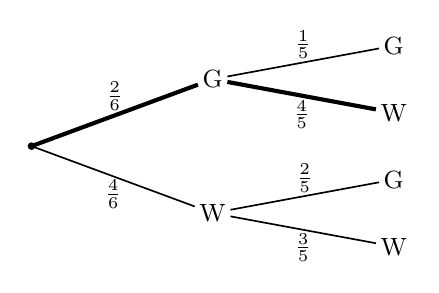
\begin{tikzpicture}[ak/.style={font=\small,inner sep=1.5pt,fill=white},wk/.style={font=\footnotesize,inner sep=1pt}]\fill (0,0) circle (1.4pt);\coordinate (s) at (0,0);\node[ak] (nG) at (2.30,0.850) {G};\node[ak] (nGG) at (4.60,1.275) {G};\node[ak] (nGW) at (4.60,0.425) {W};\node[ak] (nW) at (2.30,-0.850) {W};\node[ak] (nWG) at (4.60,-0.425) {G};\node[ak] (nWW) at (4.60,-1.275) {W};\draw[line width=1.5pt] (s) -- (nG) node[wk,above,pos=0.5] {$\frac{2}{6}$};\draw[line width=0.6pt] (nG) -- (nGG) node[wk,above,pos=0.5] {$\frac{1}{5}$};\draw[line width=1.5pt] (nG) -- (nGW) node[wk,below,pos=0.5] {$\frac{4}{5}$};\draw[line width=0.6pt] (s) -- (nW) node[wk,below,pos=0.5] {$\frac{4}{6}$};\draw[line width=0.6pt] (nW) -- (nWG) node[wk,above,pos=0.5] {$\frac{2}{5}$};\draw[line width=0.6pt] (nW) -- (nWW) node[wk,below,pos=0.5] {$\frac{3}{5}$};\end{tikzpicture}\end{varwidth}}}{}
\end{pfloesung}
\begin{pfloesung}{}
\lz{3.}{$P = \frac{1}{15}$}{Pfad Gewinn – Gewinn: $\frac{3}{10} \cdot \frac{2}{9} = \frac{6}{90} = \frac{1}{15}$}{}
\end{pfloesung}
\begin{pfloesung}{}
\lz{4.}{Nein; Beutel 2 ($\frac{15}{28} \approx 54\,\%$) ist besser als Beutel 1 ($\frac{1}{2}$)}{Nein; Beutel 1: $\frac{3}{4} \cdot \frac{2}{3} = \frac{6}{12} = \frac{1}{2}$, Beutel 2: $\frac{6}{8} \cdot \frac{5}{7} = \frac{30}{56} = \frac{15}{28} \approx 0{,}54$. Beutel 2 ist besser.}{}
\end{pfloesung}
\begin{pfloesung}{}
\lz{5b)}{a) $P = \frac{4}{7}$; b) zweimal Schwarz}{a) B – S: $\frac{4}{7} \cdot \frac{3}{6} = \frac{12}{42}$, S – B: $\frac{3}{7} \cdot \frac{4}{6} = \frac{12}{42}$; zusammen $\frac{24}{42} = \frac{4}{7}$; b) zweimal Schwarz (Pfad S – S)}{}
\end{pfloesung}
\begin{pfloesung}{}
\lz{6.}{$P = \frac{7}{15}$}{S – S: $\frac{6}{10} \cdot \frac{5}{9} = \frac{30}{90}$, W – W: $\frac{4}{10} \cdot \frac{3}{9} = \frac{12}{90}$; zusammen $\frac{42}{90} = \frac{7}{15}$}{}
\end{pfloesung}
\begin{pfloesung}{}
\lz{7.}{$P = \frac{1}{6}$}{Ali zieht keinen Joker, dann Bea den Joker: $\frac{5}{6} \cdot \frac{1}{5} = \frac{5}{30} = \frac{1}{6}$}{}
\end{pfloesung}
\begin{pfloesung}{}
\lz{8.}{Nein; beide $\frac{1}{5}$}{Nein; Jonas: $\frac{2}{10} = \frac{1}{5}$; Emma: Gewinn – Gewinn $\frac{2}{10} \cdot \frac{1}{9} = \frac{2}{90}$, Niete – Gewinn $\frac{8}{10} \cdot \frac{2}{9} = \frac{16}{90}$, zusammen $\frac{18}{90} = \frac{1}{5}$. Beide Chancen sind gleich.}{}
\end{pfloesung}
\begin{pfloesung}{}
\lz{9b)}{$P = \frac{1}{56}$}{$\frac{3}{8} \cdot \frac{2}{7} \cdot \frac{1}{6} = \frac{6}{336} = \frac{1}{56}$}{}
\end{pfloesung}
\begin{pfloesung}{}
\lz{10.}{$P = \frac{1}{5}$}{3. Stufe: nach G – G: G $\frac{2}{4}$, N $\frac{2}{4}$; nach G – N und N – G: G $\frac{3}{4}$, N $\frac{1}{4}$; nach N – N: G $\frac{4}{4}$. Genau zwei Nieten: G – N – N, N – G – N, N – N – G, je $\frac{8}{120}$; zusammen $\frac{24}{120} = \frac{1}{5}$\par\smallskip \adjustbox{max width=\linewidth,max height=4cm}{\begin{varwidth}{50cm}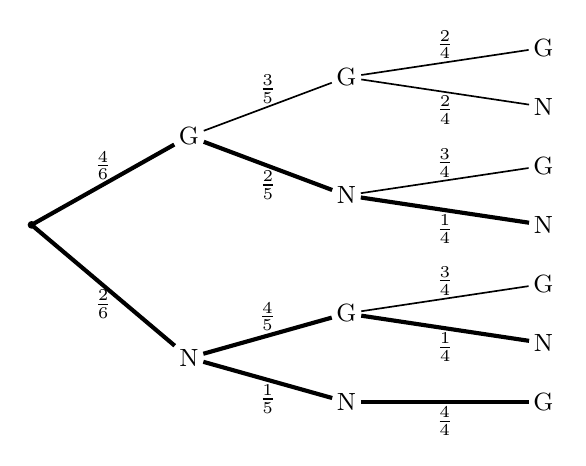
\begin{tikzpicture}[ak/.style={font=\small,inner sep=1.5pt,fill=white},wk/.style={font=\footnotesize,inner sep=1pt}]\fill (0,0) circle (1.4pt);\coordinate (s) at (0,0);\node[ak] (nG) at (2.00,1.125) {G};\node[ak] (nGG) at (4.00,1.875) {G};\node[ak] (nGGG) at (6.50,2.250) {G};\node[ak] (nGGN) at (6.50,1.500) {N};\node[ak] (nGN) at (4.00,0.375) {N};\node[ak] (nGNG) at (6.50,0.750) {G};\node[ak] (nGNN) at (6.50,0.000) {N};\node[ak] (nN) at (2.00,-1.688) {N};\node[ak] (nNG) at (4.00,-1.125) {G};\node[ak] (nNGG) at (6.50,-0.750) {G};\node[ak] (nNGN) at (6.50,-1.500) {N};\node[ak] (nNN) at (4.00,-2.250) {N};\node[ak] (nNNG) at (6.50,-2.250) {G};\draw[line width=1.5pt] (s) -- (nG) node[wk,above,pos=0.5] {$\frac{4}{6}$};\draw[line width=0.6pt] (nG) -- (nGG) node[wk,above,pos=0.5] {$\frac{3}{5}$};\draw[line width=0.6pt] (nGG) -- (nGGG) node[wk,above,pos=0.5] {$\frac{2}{4}$};\draw[line width=0.6pt] (nGG) -- (nGGN) node[wk,below,pos=0.5] {$\frac{2}{4}$};\draw[line width=1.5pt] (nG) -- (nGN) node[wk,below,pos=0.5] {$\frac{2}{5}$};\draw[line width=0.6pt] (nGN) -- (nGNG) node[wk,above,pos=0.5] {$\frac{3}{4}$};\draw[line width=1.5pt] (nGN) -- (nGNN) node[wk,below,pos=0.5] {$\frac{1}{4}$};\draw[line width=1.5pt] (s) -- (nN) node[wk,below,pos=0.5] {$\frac{2}{6}$};\draw[line width=1.5pt] (nN) -- (nNG) node[wk,above,pos=0.5] {$\frac{4}{5}$};\draw[line width=0.6pt] (nNG) -- (nNGG) node[wk,above,pos=0.5] {$\frac{3}{4}$};\draw[line width=1.5pt] (nNG) -- (nNGN) node[wk,below,pos=0.5] {$\frac{1}{4}$};\draw[line width=1.5pt] (nN) -- (nNN) node[wk,below,pos=0.5] {$\frac{1}{5}$};\draw[line width=1.5pt] (nNN) -- (nNNG) node[wk,below,pos=0.5] {$\frac{4}{4}$};\end{tikzpicture}\end{varwidth}}}{}
\end{pfloesung}
\begin{pfloesung}{}
\lz{11.}{$P = \frac{3}{8} = 37{,}5\,\%$}{Gegenteil: Nora ist auf keinem der ersten drei Plätze: $\frac{7}{8} \cdot \frac{6}{7} \cdot \frac{5}{6} = \frac{5}{8}$; $P = 1 - \frac{5}{8} = \frac{3}{8} = 37{,}5\,\%$}{}
\end{pfloesung}
\begin{pfloesung}{}
\lz{12.}{Nein; dreimal Blau ist 14-mal so wahrscheinlich}{Nein; dreimal Blau: $\frac{8}{15} \cdot \frac{7}{14} \cdot \frac{6}{13} = \frac{336}{2730} = \frac{8}{65}$; dreimal Gelb: $\frac{4}{15} \cdot \frac{3}{14} \cdot \frac{2}{13} = \frac{24}{2730} = \frac{4}{455}$; $336 : 24 = 14$, also 14-mal so wahrscheinlich.}{}
\end{pfloesung}
\begin{pfloesung}{}
\lz{13b)}{Gummibärchen essen}{– Was gegessen ist, fehlt beim 2. Zug.}{}
\end{pfloesung}
\begin{pfloesung}{}
\lz{14.}{a) $\frac{1}{9}$; b) $\frac{1}{15}$}{a) $\frac{2}{6} \cdot \frac{2}{6} = \frac{4}{36} = \frac{1}{9}$; b) $\frac{2}{6} \cdot \frac{1}{5} = \frac{2}{30} = \frac{1}{15}$}{}
\end{pfloesung}
\begin{pfloesung}{}
\lz{15.}{$P = \frac{1}{25}$}{mit Zurücklegen (das Kärtchen kommt zurück): $\frac{1}{5} \cdot \frac{1}{5} = \frac{1}{25}$}{}
\end{pfloesung}
\begin{pfloesung}{}
\lz{16.}{Sophie, um 5 Prozentpunkte ($25\,\%$ gegen $20\,\%$)}{Sophie; Glücksrad (mit Zurücklegen): $\frac{3}{6} \cdot \frac{3}{6} = \frac{1}{4} = 25\,\%$, Beutel (ohne): $\frac{3}{6} \cdot \frac{2}{5} = \frac{1}{5} = 20\,\%$; 5 Prozentpunkte mehr.}{}
\end{pfloesung}
\begin{pfloesung}{}
\lz{17.}{$P = \frac{10}{21}$}{nach G: G $\frac{4}{6}$, F $\frac{2}{6}$; nach F: G $\frac{5}{6}$, F $\frac{1}{6}$; G – G: $\frac{5}{7} \cdot \frac{4}{6} = \frac{20}{42} = \frac{10}{21}$\par\smallskip \adjustbox{max width=\linewidth,max height=4cm}{\begin{varwidth}{50cm}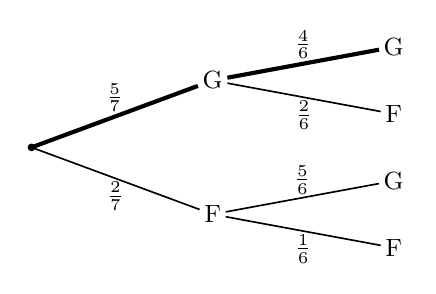
\begin{tikzpicture}[ak/.style={font=\small,inner sep=1.5pt,fill=white},wk/.style={font=\footnotesize,inner sep=1pt}]\fill (0,0) circle (1.4pt);\coordinate (s) at (0,0);\node[ak] (nG) at (2.30,0.850) {G};\node[ak] (nGG) at (4.60,1.275) {G};\node[ak] (nGF) at (4.60,0.425) {F};\node[ak] (nF) at (2.30,-0.850) {F};\node[ak] (nFG) at (4.60,-0.425) {G};\node[ak] (nFF) at (4.60,-1.275) {F};\draw[line width=1.5pt] (s) -- (nG) node[wk,above,pos=0.5] {$\frac{5}{7}$};\draw[line width=1.5pt] (nG) -- (nGG) node[wk,above,pos=0.5] {$\frac{4}{6}$};\draw[line width=0.6pt] (nG) -- (nGF) node[wk,below,pos=0.5] {$\frac{2}{6}$};\draw[line width=0.6pt] (s) -- (nF) node[wk,below,pos=0.5] {$\frac{2}{7}$};\draw[line width=0.6pt] (nF) -- (nFG) node[wk,above,pos=0.5] {$\frac{5}{6}$};\draw[line width=0.6pt] (nF) -- (nFF) node[wk,below,pos=0.5] {$\frac{1}{6}$};\end{tikzpicture}\end{varwidth}}}{}
\end{pfloesung}
\begin{pfloesung}{}
\lz{18.}{$\frac{2}{5}$}{K – K $\frac{3}{6} \cdot \frac{2}{5} = \frac{6}{30}$, Z – Z $\frac{6}{30}$; zusammen $\frac{12}{30} = \frac{2}{5}$}{}
\end{pfloesung}
\begin{pfloesung}{}
\lz{19.}{$P = \frac{1}{625} = 0{,}16\,\%$}{mit Zurücklegen: $\frac{1}{25} \cdot \frac{1}{25} = \frac{1}{625} = 0{,}16\,\%$}{}
\end{pfloesung}
\begin{pfloesung}{}
\lz{20.}{$P = \frac{17}{24} \approx 70{,}8\,\%$}{Gegenteil, keine Gewinne: $\frac{7}{10} \cdot \frac{6}{9} \cdot \frac{5}{8} = \frac{210}{720} = \frac{7}{24}$; $P = 1 - \frac{7}{24} = \frac{17}{24} \approx 70{,}8\,\%$}{}
\end{pfloesung}
\begin{pfloesung}{}
\lz{21.}{a) SK, KS, KK; b) $\frac{6}{11}$; c) Nein, nur $\frac{5}{11}$}{a) (S; K), (K; S), (K; K); b) $\frac{9}{12} \cdot \frac{8}{11} = \frac{72}{132} = \frac{6}{11} \approx 54{,}5\,\%$; c) Nein; mindestens ein Kirschmuffin: $1 - \frac{6}{11} = \frac{5}{11} \approx 45{,}5\,\%$, das ist weniger.}{}
\end{pfloesung}
\end{document}
